% ************************** Thesis Chapter3 **********************************
\chapter{ระเบียบวิธีวิจัย}
ในการทําโครงการวิจัยแอพพลิเคชั่นสำหรับวิเคราะห์วิดีโอ(video analytics) จะมีการทำงานหลากหลายส่วนมาทำงานร่วมกัน ซึ่งทำให้จำเป็นจะต้องมีระเบียบวิจัยสำหรับอธิบายภาพรวม
\subsection*{โดยในระเบียบวิจัยนี้จะมีหัวข้อ และระเบียบวิธีวิจัยดังนี้}
\begin{itemize}\setlength\itemsep{-0.3em}
	\item แผนการดำเนินงาน
	\item เครื่องมือที่ใช้ในการดำเนินงานวิจัย
	\item ภาพรวมของแอพพลิเคชั่น
	\item รายละเอียดของโมเดล
\end{itemize}
\vspace{3mm}
\section{หน้าที่ความรับผิดชอบ} 
\paragraph*{ปฐมพงศ์ สินธุ์งาม}
สร้างและทดสอบโมเดลจดจำการกระทำมนุษย์ I3D และออกแบบพร้อมทั้งสร้างระบบ Tracker
\paragraph*{ศุภกร เบญจวิกรัย}
รวบรวมฟังก์ชั่นต่างๆของแอพพลิเคชั่น และออกแบบพร้อมทั้งสร้างระบบแอพพลิเคชั่นในส่วน Selection และ Detection
\paragraph*{อุกฤษฎ์ เลิศวรรณาการ}
สร้างและทดสอบโมเดลจดจำการกระทำมนุษย์ Resnet-50 และออกแบบพร้อมทั้งสร้างระบบ Person ReID 

\vspace{3mm}
\section{แผนการดำเนินงาน}
โดยจากที่กล่าวไปตอนต้นในบทนำ
การดำเนินงานและการออกแบบการสร้าง labeling tool และระบบวิเคราะห์การกระทำของมนุษย์ในวิดีโอ มีแผนการทำงานซึ่งถูกแบ่งออกเป็นสามส่วนดังนี้ 
ส่วนแรกคือ ส่วนของการศึกษาหาความเป็นไปได้ และเทคโนโลยีในปัจจุบันที่เกี่ยวกับการสร้างแอพพลิเคชั่น และการจดจำการกระทำของมนุษย์ด้วยปัญญาประดิษฐ์ เพื่อนำมาประยุกต์ใช้กับงานวิจัยนี้
ส่วนที่สองคือ ส่วนของการออกแบบและสร้างแอพพลิเคชั่นที่ใช้ในการสร้างชุดข้อมูลสำหรับการเทรนโมเดลจากวิดีโอ
ส่วนที่สามคือ ส่วนของการออกแบบและสร้างระบบแพลตฟอร์มวิเคราะห์การกระทำของมนุษย์ได้โดยมีข้อกำหนดตามที่กล่าวไว้ในบทนำ

ในการเริ่มทำงานวิจัยนี้นั้นสิ่งจำเป็นที่ต้องทำในอันดับแรกคือการศึกษาสิ่งที่เคยมีอยู่ หรืองานวิจัยอื่นที่ทำเอาไว้แล้ว
เพื่อศึกษาและทำความเข้าใจ ข้อดี-ข้อเสีย ของเทคนิคหรือกระบวนการต่างๆ เพื่อนำมาประยุกต์ใช้กับงานวิจัยนี้
ในการศึกษาเกี่ยวกับการออกแบบและการสร้างแอพพลิเคชั่นที่ใช้ในการสร้างชุดข้อมูลสำหรับการเทรนโมเดลจากวิดีโอ
ที่มีอยู่แล้วสิ่งที่ต้องให้ความสนใจคือฟังก์ชั่นการทำงาน การออกแบบและการจัดวางองค์ประกอบต่างๆในหน้าต่าง UI
และความสะดวกในการใช้งาน จากนั้นจึงเริ่มศึกษาเกี่ยวกับแพตฟอร์มที่ใช้ในการสร้างแอพพลิเคชั่น
ส่วนการศึกษาเกี่ยวกับการสร้างระบบวิเคราะห์การกระทำมนุษย์นั้น จะมุ่งความสนใจไปที่ชุดข้อมูลสำหรับการวิเคราะห์วิดีโอ
โมเดลสำหรับการวิเคราะห์วิดีโอ เทคนิคในการสร้างโมเดล เทคโนโลยีในการทำระบบวิเคราะห์วิดีโอ
เพื่อใช้ในการออกแบบและสร้างระบบวิเคราะห์การกระทำของมนุษย์ในวิดีโอให้มีประสิทธิภาพ
ในบทนี้ก็จะกล่าวถึงกระบวนการออกแบบและการดำเนินการตามแผนที่วางเอาไว้

\clearpage
\section{การออกแบบแอพพลิเคชั่น labeling tool}
การออกแบบเครื่องมือสำหรับกำกับข้อมูลด้วยปัญญาประดิษฐ์้น ผู้วิจัยได้เลือกใช้ library PyQt และภาษาไพธอนในการพัฒนา
เนื่องจาก PyQt นั้นเป็น library ที่มีผู้พัฒนาใช้กันอย่างแพร่หลาย จึงสะดวกในการศึกษา หาข้อมูลในการสร้างหรือแก้ไข
อีกทั้งยังเป็น library ที่สามารถพัฒนาด้วยภาษาไพธอนได้ และใช้งานง่าย สามารถปรับปรุงแก้ไขได้สะดวก

\subsection{เครื่องมือสำหรับกำกับข้อมูลด้วยปัญญาประดิษฐ์}
แอพพลิเคชั่นแบ่งการทำงานออกเป็นสี่ส่วนประกอบด้วยกระบวนการ Select, Detect, Track และ Label
เพื่อช่วยแบ่งเบาภาระของผู้พัฒนาในการสร้างชุดข้อมูลสำหรับสร้างโมเดลจากข้อมูลประเภทวิดีโอ โดยกระบวนการ Select
จะต้องสามารถตัดวิดีโอส่วนที่ไม่มีมนุษย์อยู่ออกจากวิดีโอได้ จากนั้นกระบวนการ Detect จะต้องหาตำแหน่งของมนุษย์ภายในวิดีโอได้
แล้วใช้กระบวนการ Track ทำนายตำแหน่งต่อไปของมนุษย์ข้อมูลตำแหน่งของมนุษย์ที่ได้จากกระบวนการ Detect
และกระบวนการ Label นั้นต้องสามารถทำนายการกระทำพื้นฐานของมนุษย์ได้ เช่น ยืน เดิน นั่ง กินข้าว หรือ นอน เป็นต้น 
โดยทุกส่วนการทำงานมนุษย์ต้องสามารถทำงานร่วมกับปัญญาประดิษฐ์ได้
ดังรูปที่ \ref{fig:labeling_overview}

\begin{figure}[!ht]
    \centering
    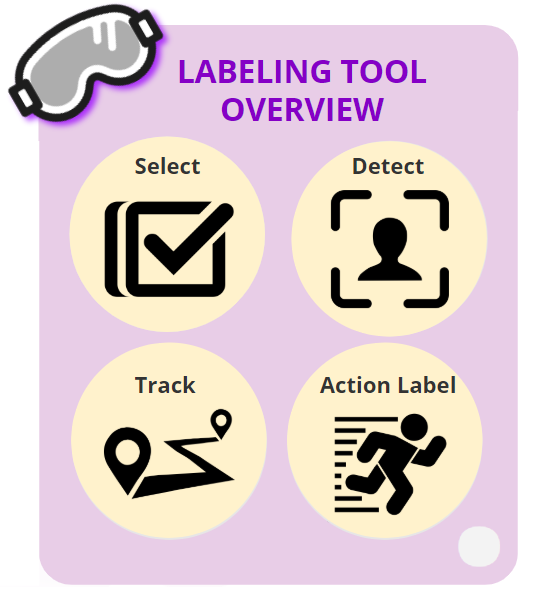
\includegraphics[width=0.5\textwidth]{chapter3/images/3_6/labelingToolOverview.png}
    \caption{กระบวนการหลักของเครื่องมือสำหรับกำกับข้อมูลด้วยปัญญาประดิษฐ์}
    \label{fig:labeling_overview}
\end{figure}
\clearpage

\subsection*{โดยแต่ละกระบวนการจะมีรายละเอียดดังนี้}
\subsubsection{Select}
กระบวนการ Select จะต้องสามารถรับวิดีโอเข้ามา แล้วตัดวิดีโอในช่วงที่ไม่มนุษย์อยู่ในเฟรมออกได้อัตโนมัติด้วยปัญญาประดิษฐ์
แต่เนื่องจากการประมวลผลทุกเฟรมในวิดีโอนั้นจะทำให้เสียเวลามากเกินไป จึงใช้วิธีการเลือกตัวอย่างเฟรมด้วยอัตราคงที่ (สามารถกำหนดได้)
ซึ่งเรียกว่าเฟรมเหล่านี้ว่า คีย์เฟรม จากนั้นใช้ปัญญาประดิษฐ์ประมวลผลคีย์เฟรมที่เหล่านั้น 
เพื่อลดระยะเวลาในการประมวลผลลง และมนุษย์จะต้องสามารถแก้ไขข้อผิดพลาดของปัญญาประดิษฐ์ได้ 
เพื่อเพิ่มคุณภาพของชุดข้อมูล จึงออกแบบหน้าต่างได้ดังรูปที่ \ref{fig:SelectDraft}

\begin{figure}[!ht]
    \centering
    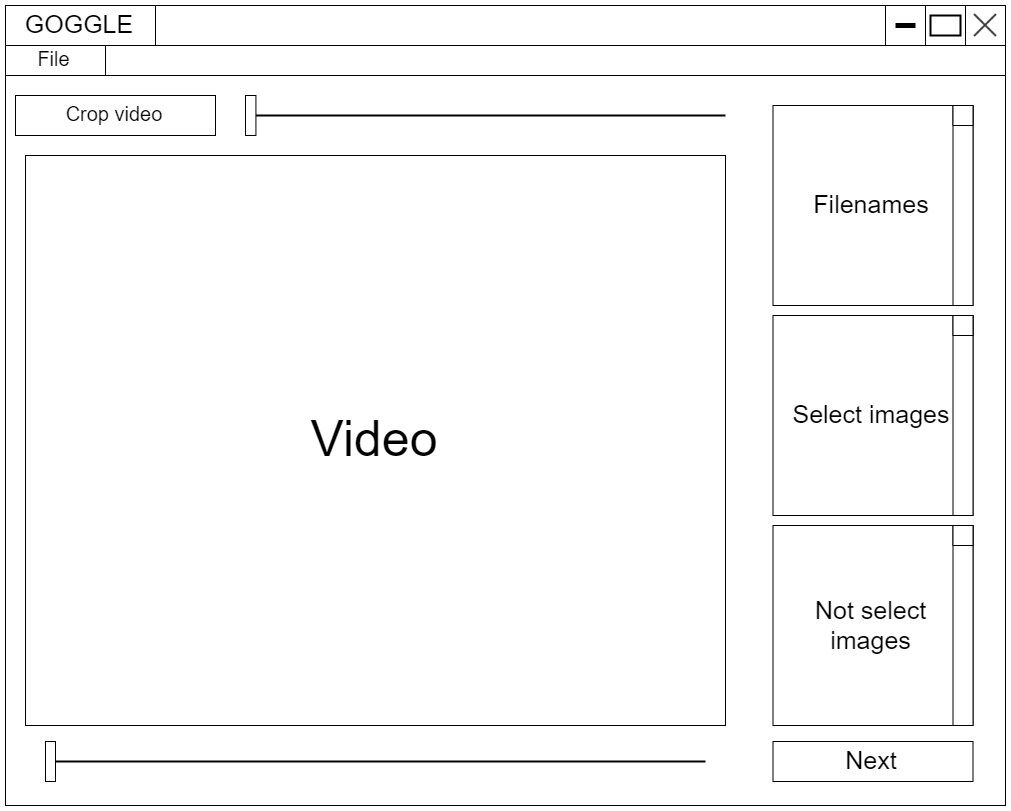
\includegraphics[width=1\textwidth]{chapter3/images/3_6/SelectDraft.png}
    \caption{หน้าต่าง Select ของเครื่องมือสำหรับกำกับข้อมูลด้วยปัญญาประดิษฐ์}
    \label{fig:SelectDraft}
\end{figure}
\clearpage
\begin{figure}[!ht]
    \centering
    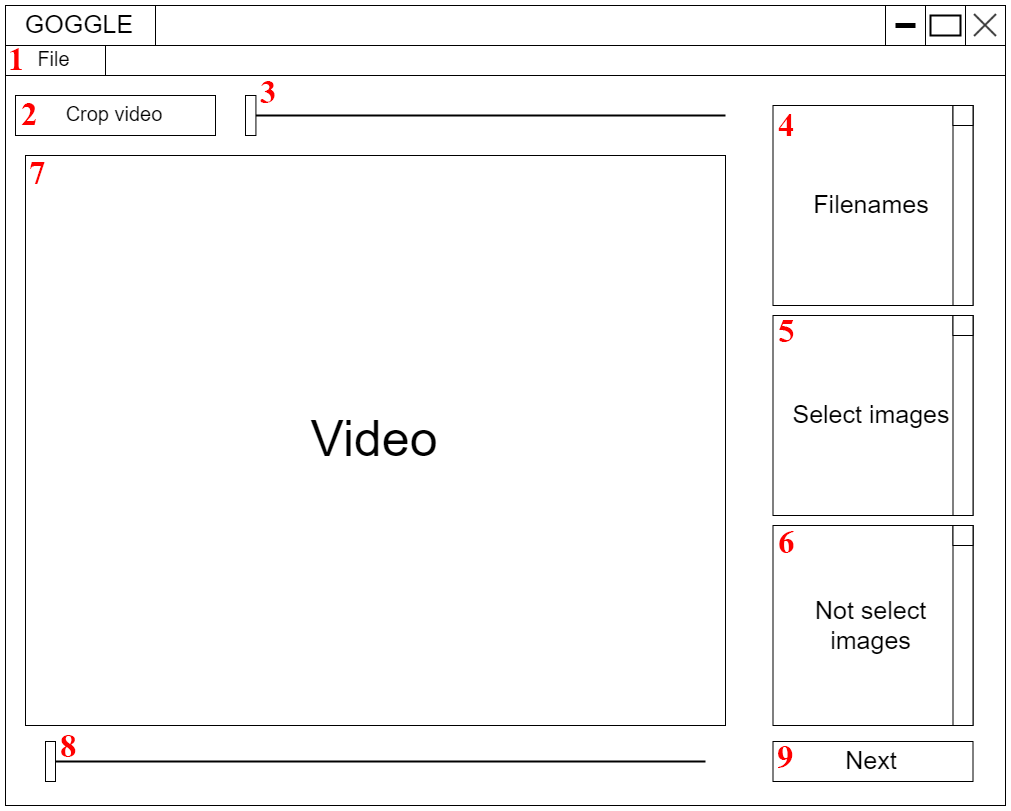
\includegraphics[width=1\textwidth]{chapter3/images/3_6/SelectDraft_point.png}
    \caption{ตำแหน่งของแต่ละวิดเจ็ตในหน้าต่าง Select}
    \label{fig:SelectDraft_point}
\end{figure}
โดยที่แต่ละวิดเจ็ตตามหมายเลขที่กำหนดตามรูปที่ \ref{fig:SelectDraft_point} มีรายละเอียดดังนี้
\begin{enumerate}
	\setlength\itemsep{-0.25em}
	\item หมายเลข 1 คือปุ่มสำหรับเลือกไฟล์วิดีโอที่ต้องการจากในคอมพิวเตอร์เข้ามาในโปรแกรม
    \item หมายเลข 2 คือปุ่มสำหรับสั่งให้ระบบทำการสร้างคีย์เฟรมขึ้นมา แล้วใช้ปัญญาประดิษฐ์ประมวลผลเพื่อแยกว่าคีย์เฟรมไหนมีคนอยู่ และคีย์เฟรมไหนไม่มีคนอยู่แบบอัตโนมัติ
    \item หมายเลข 3 คือแถบเลื่อนเพื่อกำหนดความถี่ในการหยิบคีย์เฟรม โดยจะมีช่วงอยู่ที่ 1 เฟรมต่อวินาที จนถึง อัตราเฟรมต่อวินาทีสูงสุดของวิดีโอที่รับเข้ามา
	\item หมายเลข 4 คือกล่องสำหรับแสดงชื่อวิดีโอที่รับเข้ามาในโปรแกรมเพื่อเลือกเข้ามาใช้ในการประมวลผล
	\item หมายเลข 5 คือกล่องสำหรับแสดงว่าคีย์เฟรมใดมีมนุษย์อยู่ในเฟรม โดยที่ผู้ใช้งานสามารถตรวจสอบความถูกต้องและแก้ไขข้อผิดพลาดของปัญญาประดิษฐ์ได้
	\item หมายเลข 6 คือกล่องสำหรับแสดงว่าคีย์เฟรมใดไม่มีมนุษย์อยู่ในเฟรม โดยที่ผู้ใช้งานสามารถตรวจสอบความถูกต้องและแก้ไขข้อผิดพลาดของปัญญาประดิษฐ์ได้
	\item หมายเลข 7 คือหน้าต่างสำหรับแสดงเฟรมที่เลือกจากหมายเลข 5 หมายเลข 6 หรือหมายเลข 8
	\item หมายเลข 8 คือแถบเลื่อนสำหรับเลื่อนดูคีย์เฟรมทั้งหมดที่ระบบสร้างขึ้น
	\item หมายเลข 9 คือปุ่มสำหรับไปกระบวนการต่อไปหลังจากระบบประมวลผลเสร็จแล้ว
\end{enumerate}
\clearpage

\subsubsection{Detect}
กระบวนการ Delect จะต้องสามารถรับคีย์เฟรมจากกระบวนการ Select มาประมวลผลด้วยปัญญาประดิษฐ์เพื่อหาตำแหน่งของมนุษย์ที่อยู่ในคีย์เฟรม 
แล้วสร้างกรอบสี่เหลี่ยมครอบบริเวณดังกล่าวได้ในแบบอัตโนมัติ เพื่อแบ่งเบาภาระผู้ใช้ในการที่ต้องสร้างกรอบสี่เหลี่ยมครอบตำแหน่งของมนุษย์ด้วยตัวเอง
และผู้ใช้ต้องสามารถสร้างหรือลบกรอบสี่เหลี่ยมได้ด้วยตัวเองสำหรับแก้ไขความผิดพลาดของปัญญาประดิษฐ์ เพื่อเพิ่มคุณภาพของชุดข้อมูล
จึงออกแบบหน้าต่างได้ดังรูปที่ \ref{fig:DetectDraft}
\begin{figure}[!ht]
    \centering
    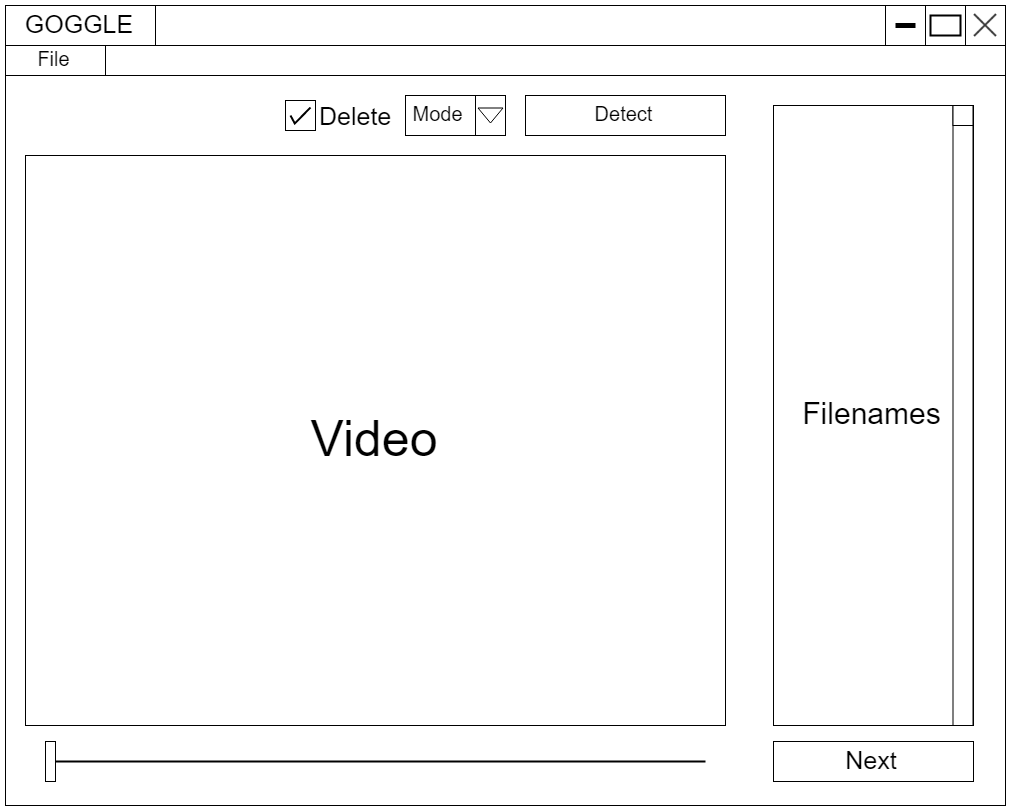
\includegraphics[width=1\textwidth]{chapter3/images/3_6/DetectDraft.png}
    \caption{หน้าต่าง Detect ของเครื่องมือสำหรับกำกับข้อมูลด้วยปัญญาประดิษฐ์}
    \label{fig:DetectDraft}
\end{figure}
\clearpage
\begin{figure}[!ht]
    \centering
    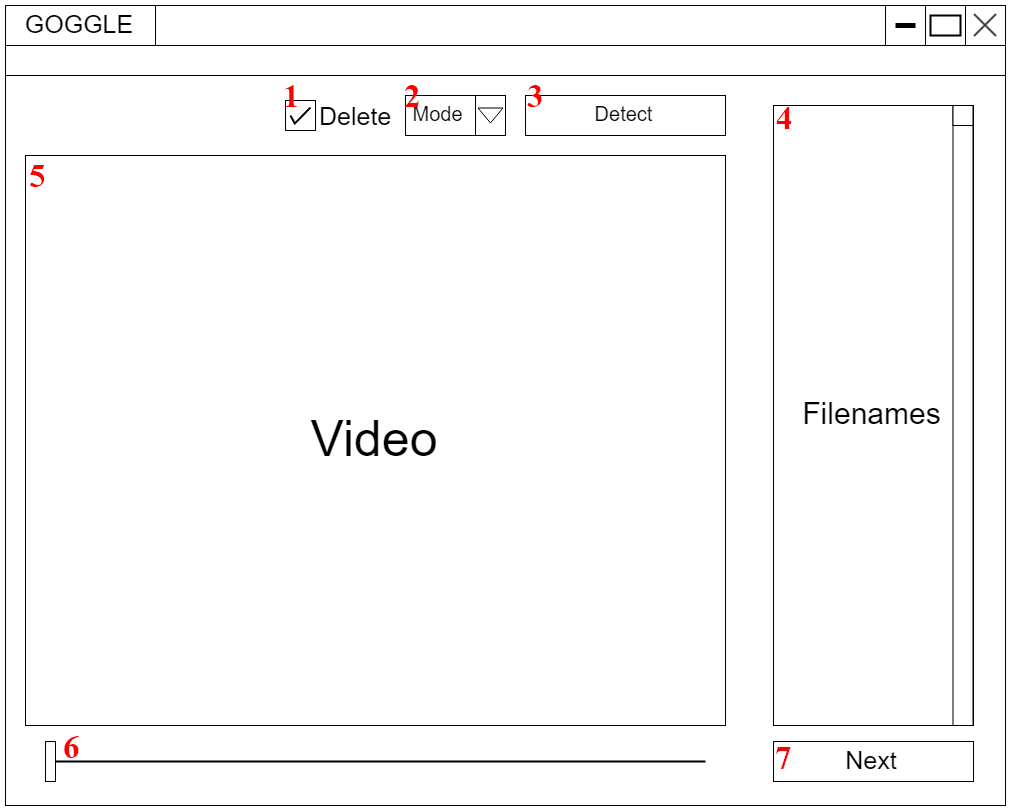
\includegraphics[width=1\textwidth]{chapter3/images/3_6/DetectDraft_point.png}
    \caption{ตำแหน่งของแต่ละวิดเจ็ตในหน้าต่าง Detect}
    \label{fig:DelectDraft_point}
\end{figure}
โดยที่แต่ละวิดเจ็ตตามหมายเลขที่กำหนดตามรูปที่ \ref{fig:DelectDraft_point} มีรายละเอียดดังนี้
\begin{enumerate}
	\setlength\itemsep{-0.25em}
    \item หมายเลข 1 คือช่องสำหรับกดเพื่อเปลี่ยนระบบจากสร้างกรอบสี่เหลี่ยมในแบบแก้ไขด้วยตนเองเป็นลบกรอบสี่เหลี่ยมแทน
    \item หมายเลข 2 คือช่องสำหรับเลือกว่าจะใช้ระบบแบบใด ระหว่างแบบอัตโนมัติและแบบแก้ไขด้วยตนเอง
    \item หมายเลข 3 คือปุ่มสำหรับสั่งให้ระบบทำการตรวจหาตำแหน่งของมนุษย์ในคีย์เฟรมทั้งหมดแล้วสร้างกรอบสี่เหลี่ยมขึ้นมาครอบบริเวณที่กำหนด
	\item หมายเลข 4 คือกล่องสำหรับแสดงคีย์เฟรมทั้งหมด
	\item หมายเลข 5 คือหน้าต่างสำหรับแสดงเฟรมที่เลือกจากหมายเลข 4 หรือหมายเลข 6
	\item หมายเลข 6 คือแถบเลื่อนสำหรับเลื่อนดูคีย์เฟรมทั้งหมดที่มี เพื่อตรวจสอบความถูกต้องของปัญญาประดิษฐ์
	\item หมายเลข 7 คือปุ่มสำหรับไปกระบวนการต่อไปหลังจากระบบประมวลผลเสร็จแล้ว
\end{enumerate}
\clearpage

\subsubsection{Track}
เนื่องจากกระบวนการ Detect นั้นจะทำเฉพาะในคีย์เฟรมทำให้ในเฟรมอื่นๆนอกเหนือจากนั้นจะไม่มีกรอบสี่เหลี่ยมอยู่
ดังนั้นกระบวนการ Track จึงต้องสามารถทำนายตำแหน่งต่อไปของมนุษย์แล้วสร้างกรอบสี่เหลี่ยมขึ้นมาบนเฟรมระหว่างคีย์เฟรมทั้งหมดได้โดยอัตโนมัติ
เพื่อสร้างข้อมูลตำแหน่งของมนุษย์ในเฟรมเหล่านั้น และผู้ใช้ต้องสามารถสร้างหรือลบกรอบสี่เหลี่ยมได้ด้วยตัวเองสำหรับแก้ไขความผิดพลาดของอัลกอริทึม
จึงออกแบบหน้าต่างได้ดังรูปที่ \ref{fig:TrackDraft}
\begin{figure}[!ht]
    \centering
    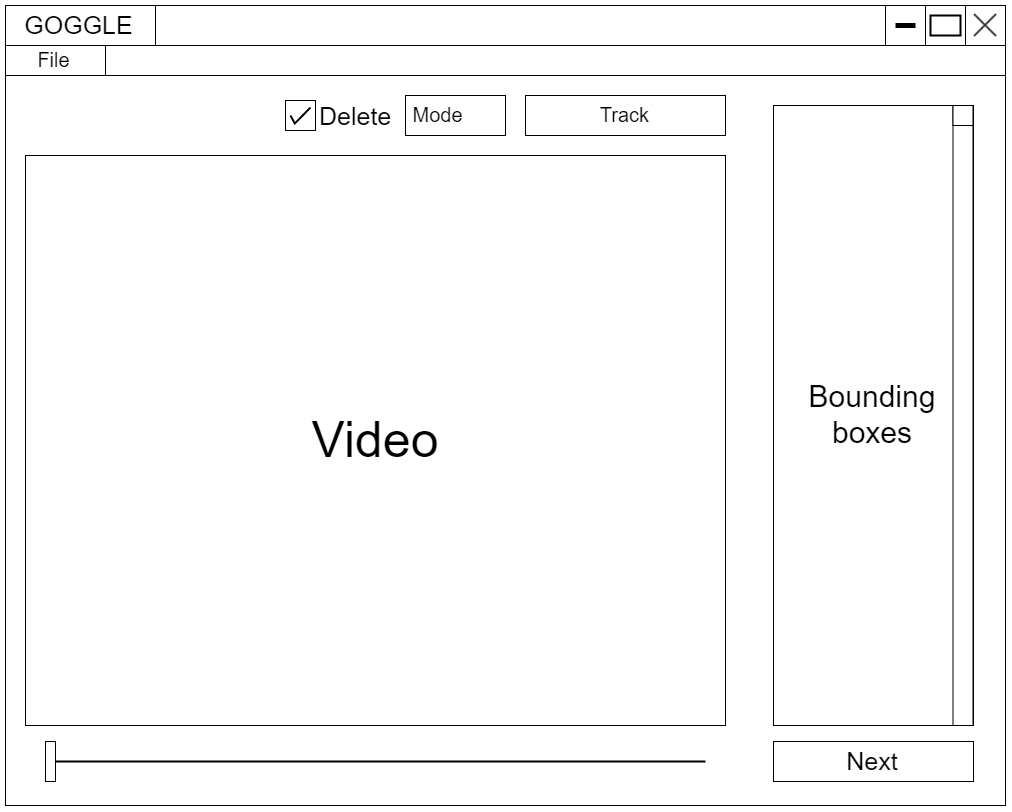
\includegraphics[width=1\textwidth]{chapter3/images/3_6/TrackDraft.png}
    \caption{หน้าต่าง Track ของเครื่องมือสำหรับกำกับข้อมูลด้วยปัญญาประดิษฐ์}
    \label{fig:TrackDraft}
\end{figure}
\clearpage
\begin{figure}[!ht]
    \centering
    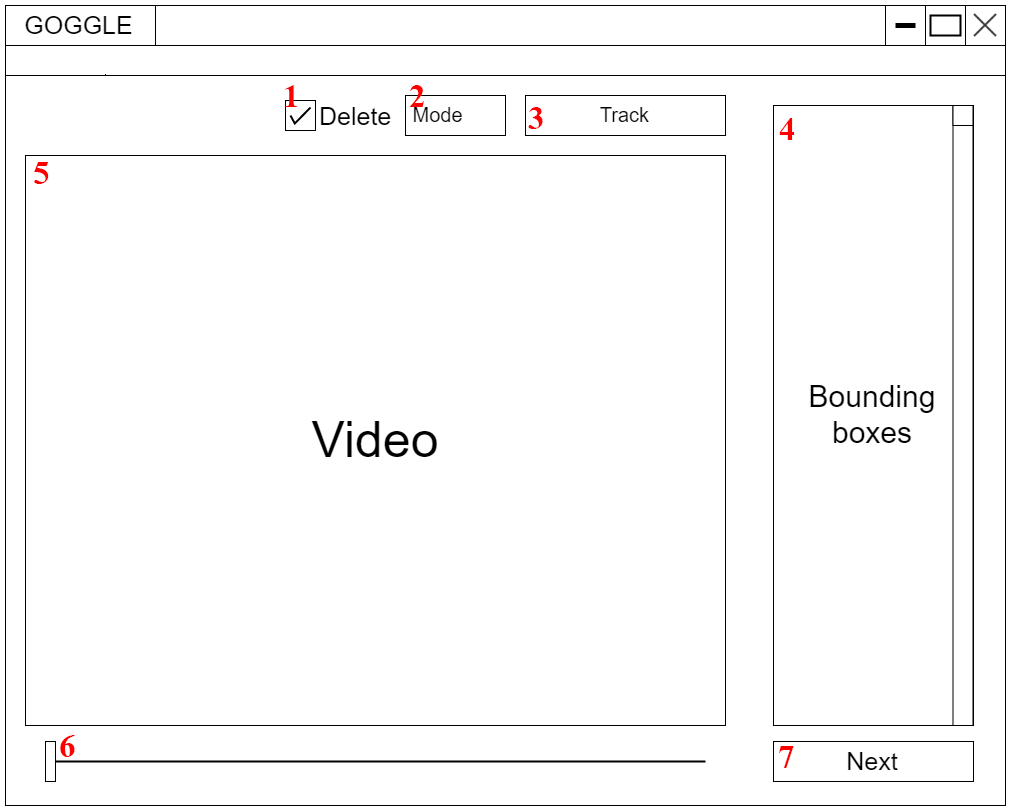
\includegraphics[width=1\textwidth]{chapter3/images/3_6/TrackDraft_point.png}
    \caption{ตำแหน่งของแต่ละวิดเจ็ตในหน้าต่าง Track}
    \label{fig:TrackDraft_point}
\end{figure}
โดยที่แต่ละวิดเจ็ตตามหมายเลขที่กำหนดตามรูปที่ \ref{fig:TrackDraft_point} มีรายละเอียดดังนี้
\begin{enumerate}
	\setlength\itemsep{-0.25em}
    \item หมายเลข 1 คือช่องสำหรับกดเพื่อเปลี่ยนระบบจากสร้างกรอบสี่เหลี่ยมในแบบแก้ไขด้วยตนเองเป็นลบกรอบสี่เหลี่ยมแทน
    \item หมายเลข 2 คือช่องสำหรับเลือกว่าจะใช้ระบบแบบใด ระหว่างแบบอัตโนมัติและแบบแก้ไขด้วยตนเอง
    \item หมายเลข 3 คือปุ่มสำหรับสั่งให้ระบบทำการตรวจหาตำแหน่งของมนุษย์ในเฟรมระหว่างคีย์เฟรมทั้งหมดแล้วสร้างกรอบสี่เหลี่ยมขึ้นมาครอบบริเวณที่กำหนด
	\item หมายเลข 4 คือกล่องสำหรับแสดงกรอบสี่เหลี่ยมทั้งหมดที่อยู่ในเฟรม
	\item หมายเลข 5 คือหน้าต่างสำหรับแสดงเฟรมที่เลือกจากหมายเลข 6
	\item หมายเลข 6 คือแถบเลื่อนสำหรับเลื่อนดูเฟรมทั้งหมดที่มี เพื่อตรวจสอบความถูกต้องของอัลกอริทึม
	\item หมายเลข 7 คือปุ่มสำหรับไปกระบวนการต่อไปหลังจากระบบประมวลผลเสร็จแล้ว
\end{enumerate}
\clearpage

\subsubsection{Label}
กระบวนการ Label นั้นต้องสามารถทำนายว่าการกระทำของมนุษย์ที่อยู่ในแต่ละเฟรมว่าคืออะไรได้โดยอัตโนมัติด้วยปัญญาประดิษฐ์
และผู้ใช้จะต้องสามารถแก้ไขข้อผิดพลาดของปัญญาประดิษฐ์ได้หากมีการทำนายที่ผิดพลาดเกิดขึ้น
หรือถ้าหากผู้ใช้ต้องการเพิ่มการกระทำที่ไม่ได้มีอยู่ในชุดการกระทำพื้นฐานที่มีอยู่แล้วของปัญญาประดิษฐ์ ผู้ใช้ก็สามารถเพิ่มการกระทำนั้นเข้ามาได้
จึงออกแบบหน้าต่างได้ดังรูปที่ \ref{fig:ActionLabelDraft}
\begin{figure}[!ht]
    \centering
    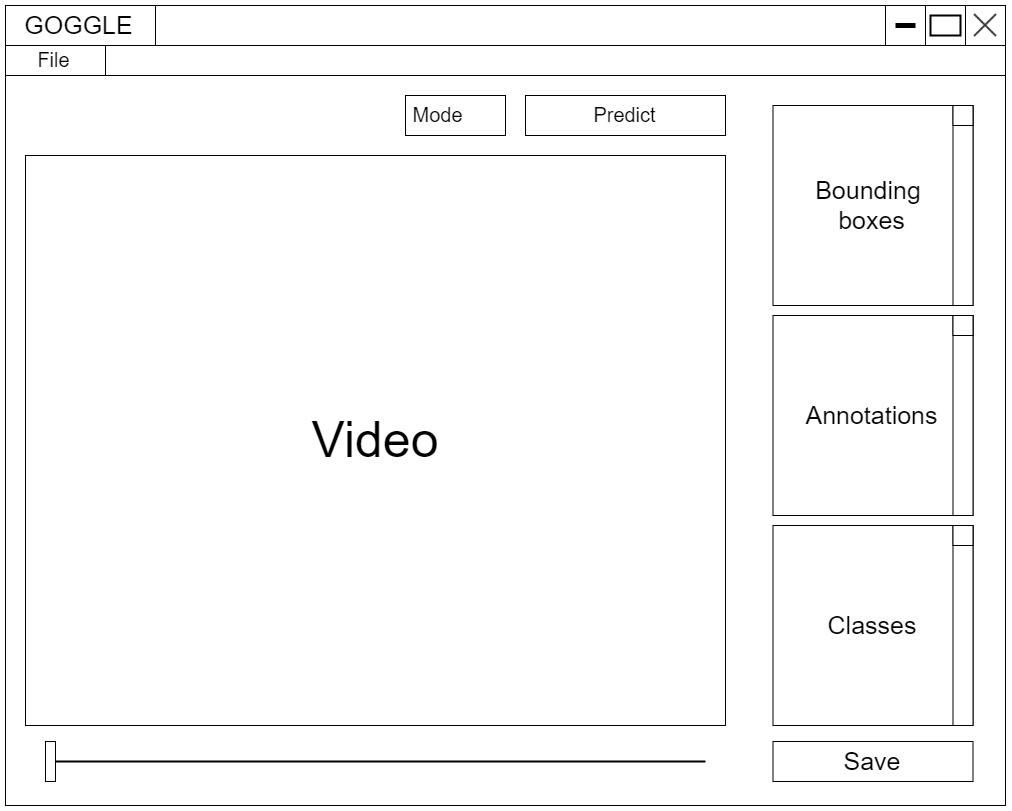
\includegraphics[width=1\textwidth]{chapter3/images/3_6/ActionLabelDraft.png}
    \caption{หน้าต่าง Label ของเครื่องมือสำหรับกำกับข้อมูลด้วยปัญญาประดิษฐ์}
    \label{fig:ActionLabelDraft}
\end{figure}
\clearpage
\begin{figure}[!ht]
    \centering
    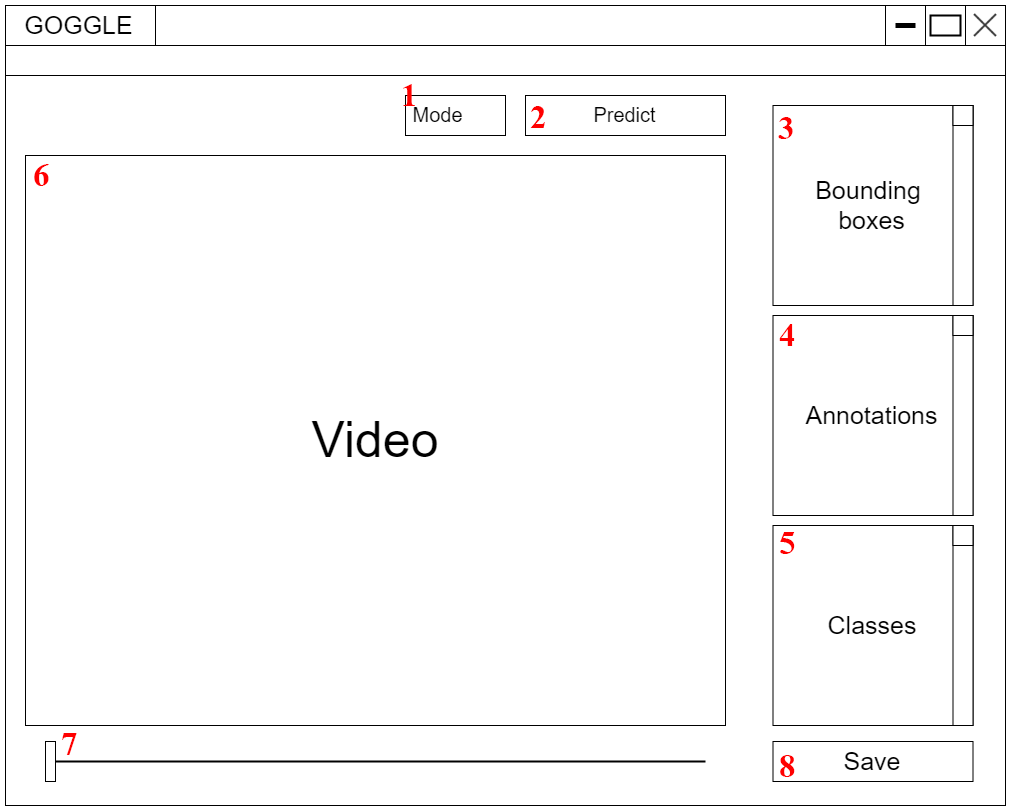
\includegraphics[width=1\textwidth]{chapter3/images/3_6/ActionLabelDraft_point.png}
    \caption{ตำแหน่งของแต่ละวิดเจ็ตในหน้าต่าง Label}
    \label{fig:ActiobLabelDraft_point}
\end{figure}
โดยที่แต่ละวิดเจ็ตตามหมายเลขที่กำหนดตามรูปที่ \ref{fig:TrackDraft_point} มีรายละเอียดดังนี้
\begin{enumerate}
	\setlength\itemsep{-0.25em}
    \item หมายเลข 1 คือช่องสำหรับเลือกว่าจะใช้ระบบแบบใด ระหว่างแบบอัตโนมัติและแบบแก้ไขด้วยตนเอง
    \item หมายเลข 2 คือปุ่มสำหรับสั่งให้ระบบทำนายการกระทำของมนุษย์ในทุกๆเฟรม
    \item หมายเลข 3 คือกล่องสำหรับแสดงกรอบสี่เหลี่ยมทั้งหมดที่อยู่ในเฟรมที่เลือก
	\item หมายเลข 4 คือกล่องสำหรับแสดงการกระทำของมนุษย์แต่ละคนที่อยู่ในเฟรมที่เลือก โดยจะเรียงลำดับคู่กับกรอบสี่เหลี่ยมที่อยู่ในช่องหมายเลข 3
    \item หมายเลข 5 คือกล่องสำหรับแสดงชุดการกระทำที่ปัญญาประดิษฐ์มีอยู่แล้ว ซึ่งในการทำงานแบบแก้ไขด้วยตนเองนั้น จะสามารถค้นหาการกระทำที่มีอยู่แล้วได้ 
    และหากคำที่ใส่เข้ามานั้นไม่มีอยู่ในชุดการกระทำก็จะเป็นการเพิ่มการกระทำนั้นเข้ามาแทน
	\item หมายเลข 6 คือหน้าต่างสำหรับแสดงเฟรมที่เลือกจากหมายเลข 7
	\item หมายเลข 7 คือแถบเลื่อนสำหรับเลื่อนดูเฟรมทั้งหมดที่มี เพื่อตรวจสอบความถูกต้องของปัญญาประดิษฐ์
	\item หมายเลข 8 คือปุ่มสำหรับสร้างไฟล์ xml ของทุกๆเฟรมสำหรับใช้ในการสร้างโมเดลโดยรายละเอียดข้อมูลภายในไฟล์ xml จะอยู่ในหัวข้อ \ref{sec:XMLInfo}
\end{enumerate}
\clearpage

\subsubsection{รายละเอียดข้อมูลภายในไฟล์ xml}
\label{sec:XMLInfo}
ไฟล์ xml นั้นเป็นรูปแบบที่นิยมใช้ในการเก็บข้อมูลสำหรับการสร้างโมเดลประเภทตรวจจับวัตถุ
โดยจะเก็บข้อมูลในรูปแบบของ PASCAL VOC ที่นิยมใช้ในการสร้างโมเดลด้วย Tensorflow โดยภายในไฟล์จะมีข้อมูลดังรูปที่ \ref{fig:XMLFormat}
\begin{figure}[!ht]
    \centering
    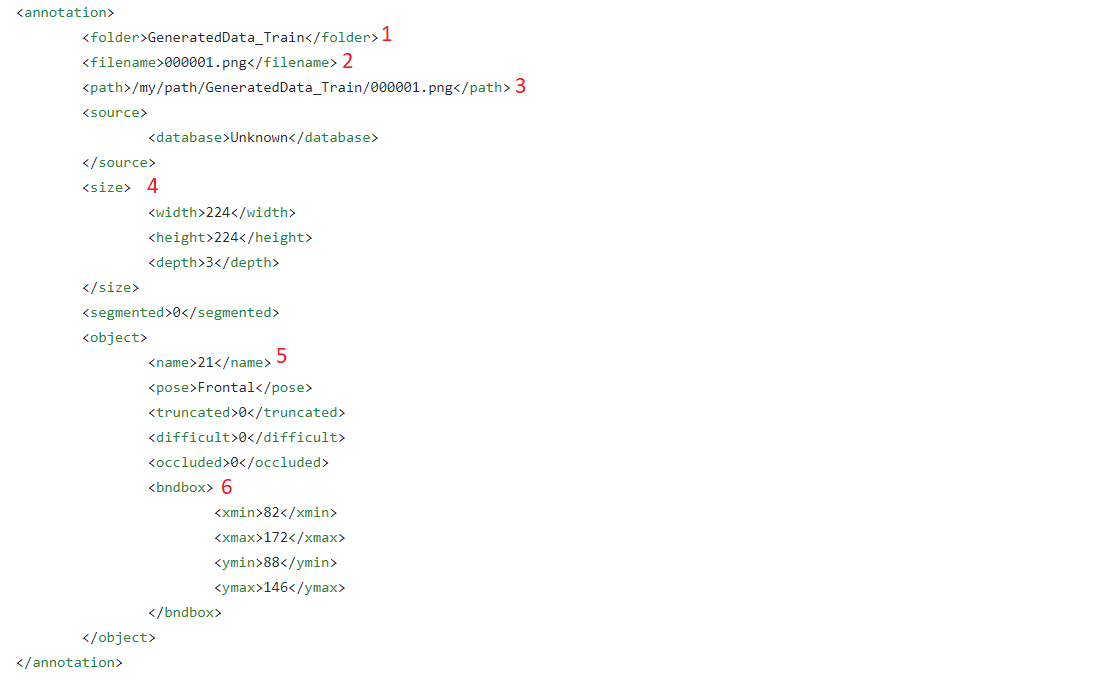
\includegraphics[width=1\textwidth]{chapter3/images/3_6/XMLFormat.png}
    \caption{ตัวอย่างข้อมูลภายในไฟล์ xml}
    \label{fig:XMLFormat}
\end{figure}
โดยข้อมูลส่วนสำคัญของรูปแบบนี้นั้นจะถูกใส่หมายเลขกำกับไว้ซึ่งแต่ละหมายเลขนั้นหมายถึง
\begin{enumerate}
	\setlength\itemsep{-0.25em}
    \item หมายเลข 1 คือชื่อโฟลเดอร์ที่เก็บไฟล์รูปภาพที่เกี่ยวข้องกับไฟล์ xml นี้อยู่
    \item หมายเลข 2 คือชื่อไฟล์ที่เกี่ยวข้องกับไฟล์ xml นี้
    \item หมายเลข 3 คือเส้นทางในคอมพิวเตอร์ (directory path) ของไฟล์รูปภาพที่เกี่ยวข้องกับไฟล์ xml นี้
    \item หมายเลข 4 คือขนาดและมิติของรูปภาพ ซึ่งจะประกอบด้วยความกว้าง (width) ความยาว (height) และจำนวนช่องสี (depth) 
    โดยที่จำนวนช่องสีที่มีความลึก 3 มักจะหมายถึงภาพสี RGB และจำนวนช่องสีที่มีความลึก 2 จะหมายถึงภาพขาวดำ (gray scale)
	\item หมายเลข 5 คือ label ของวัตถุหรืออย่างอื่น ที่อยู่ในกรอบสี่เหลี่ยมที่ถูกกำหนดไว้ในส่วนของหมายเลข 6
	\item หมายเลข 6 คือ กรอบสี่เหลี่ยมที่ครอบวัตถุที่สนใจ เช่นมนุษย์ เป็นต้น
\end{enumerate}

\clearpage
\section{การออกแบบระบบวิเคราะห์การกระทำของมนุษย์}
การออกแบบโปรแกรมด้วย ROS ของหุ่นยนต์ฮิวมานอยด์ UTHAI นั้น
ผู้วิจัยได้วางการทำงานโดย เริ่มจากการสร้างแบบจำลองเพื่อใช้ในการจำลองการทำงานของหุ่นยนต์ฮิวมานอยด์ UTHAI
โดยการจัดสร้างไฟล์ URDF ขึ้น ทดสอบการเคลื่อนไหวของหุ่นยนต์ในการแสดงผลด้วยภาพผ่านโปรแกรม RViz
ทดสอบการสั่งการดิจิตอลเซอร์โว ทดสอบการอ่านตำแหน่งจากดิจิตอลเซอร์โว
ทดสอบการส่งค่าตำแหน่งจากดิจิตอลเซอร์โวไปประมวลผลหาจุดศูนย์กลางมวลในโปรแกรม MATLAB
และเขียนโปรแกรมอ่านค่าเซนเซอร์ตรวจการสัมผัสพื้น

\vspace{20pt}
\subsection{กำหนดพิกัดเฟรมให้กับหุ่นยนต์ฮิวมานอยด์}
การกำหนดเฟรมให้กับหุ่นยนต์ฮิวมานอยด์ UTHAI นั้น ในวิทยานิพนธ์เล่มนี้ ผู้วิจัยจะใช้หลักตามของ
ROS Enhancement Proposals (REPs)\footnote{http://www.ros.org/reps/rep-0000.html}
ซึ่งการใช้หลักการนี้จะทำให้ การเขียนเป็นระบบระเบียบสามารถหยิบเครื่องมือต่างๆ
ที่สร้างขึ้นมาใช้งานร่วมกันได้ และช่วยทำให้เกิดความเข้าใจเวลาสื่อสาร

\paragraph*{base\_link}
เป็นเฟรมที่ติดอยู่กับฐานของหุ่นยนต์ฮิวมานอยด์ โดยจะติดตำแหน่งหรือมุมเอียงใดก็ได้
โดยส่วนใหญ่แล้วจะติดเฟรม base\_link ไว้ที่สะโพกของหุ่นยนต์

\paragraph*{base\_footprint}
เป็นเฟรมที่แสดงว่าหุ่นยนต์อยู่ตรงไหนเมื่อเทียบกับโลก โดยจะมีระดับอยู่ที่จุดต่ำสุดของฝ่าเท้า $z = min(l\_sole\_z,r\_sole\_z)$
โดย $l\_sole\_z$ และ $r\_sole\_z$ คือความสูงของฝ่าเท้า

\paragraph*{l\_wrist, r\_wrist}
เป็นเฟรมที่บอกตำแหน่งและมุมเอียงของแขนซ้ายและขวาของหุ่นยนต์ฮิวมานอยด์ โดยไม่ต้องคำนึงถึงการติดตั้งอุปกรณ์ใดๆเข้าไปที่ปลายแขนของหุ่นยนต์ฮิวมานอยด์

\paragraph*{l\_gripper, r\_gripper}
เป็นเฟรมที่บอกตำแหน่งและมุมเอียงของที่ปลายแขน (End effector) ถ้ามือจับอุปกรณ์อยู่ เฟรมนี้จะใช้ในการอ้างอิงตำแหน่งของอุปกรณ์นั้นๆ
แต่ในวิทยานิพนธ์นี้ ไม่ได้ใช้แขนของหุ่นยนต์ในการหยิบจับเครื่องมือหรือวัตถุ จึงไม่ได้ใช้เฟรมนี้

\paragraph*{l\_ankle, r\_ankle}
เป็นเฟรมที่บอกตำแหน่งและมุมเอียงของขาซ้ายและขวาโดยไม่ได้คำนึงว่าจุดรับน้ำหนักของตัวอยู่ที่ไหน

\paragraph*{l\_sole, r\_sole}
เป็นเฟรมที่บอกตำแหน่งและมุมเอียงของขาซ้ายและขวาที่รองรับน้ำหนักตัวอยู่
โดยจะบอกการฉายลงในระนาบของ $X$, $Y$ ที่สัมผัสพื้นและ $Z$ จะอยู่ระดับเดียวกับพื้นสัมผัส

\paragraph*{l\_toe, r\_toe}
เป็นเฟรมที่บอกตำแหน่งและมุมเอียงของปลายเท้าซ้ายและขวา

\paragraph*{gaze}
เป็นเฟรมที่บอกตำแหน่งและมุมเอียงของหัว โดยการเอียงนั้นจะบอกทิศทางของหัว โดยไม่ได้สนใจเซนเซอร์ว่าจะติดตั้งอย่างไร
แต่ในวิทยานิพนธ์นี้ หุ่นยนต์ฮิวมานอยด์ UTHAI ไม่มีหัว จึงไม่ได้ใช้เฟรมนี้

\paragraph*{torso}
เป็นเฟรมที่ติดอยู่กับลำตัวช่วงล่างของหุ่นยนต์ฮิวมานอยด์ โดยจะเป็นเฟรมที่ใช้เชื่อม ขา แขน ตัว หัว เข้าเอาไว้ด้วยกัน





%%%%%%%%%%%%%%%%%%%%%%%%%%%%%%%%%%%%%%%%%%%%%%%%%%%%%%%%%%%%%%%%%%%%%%%%%%%%%%%
\clearpage
\subsection{การแปลงข้อมูลให้อยู่ในรูปแบบ URDF}
เมื่อออกแบบโครงสร้างของหุ่นยนต์ฮิวมานอยด์ UTHAI ด้วยโปรแกรม Solidworks เสร็จแล้ว
ต่อไปเป็นการนำเอาไฟล์ STL ออกมาเพื่อใช้ในการทำระบบจำลองการทำงานของหุ่นยนต์
โดยการใช้งานระบบจำลองเนื่องจากทำให้ผู้วิจัยสามารถที่จะเห็นการทำงานของหุ่นยนต์ฮิวมานอยด์ได้
การสร้างแบบจำลองโดยการใช้เครื่องมือที่มาพร้อมกับ ROS ด้วยโมดูล URDF

\subsubsection{แพกเกจ ROS สำหรับสร้างแบบจำลอง}
ROS ได้ให้เครื่องมือที่ช่วยให้ สามารถที่จะสร้างแบบจำลองของหุ่นยนต์ฮิวมานอยด์สามมิติได้
เครื่องมือใน ROS ที่ชื่อว่า robot\_model ภายในมีแพกเกจต่างๆที่ใช้สำหรับสร้างแบบจำลองของหุ่นยนต์สามมิติอยู่อย่างครบถ้วน
ทำให้เราสามารถทำงานได้สะดวก และรวดเร็วมากขึ้น

\paragraph*{urdf}
เป็นหนึ่งในหลายแพกเกจที่อยู่ใน robot\_model, URDF เป็นไฟล์ XML ที่เอาไว้ใช้บอกลักษณะทางกายภาพของหุ่นยนต์ ซึ่งย่อมาจาก Unified Robot Description Format (URDF)
การบอกโครงสร้างของหุ่นยนต์ด้วย URDF จะใช้การบอกเป็นโครงสร้างต้นไม้ของก้านต่อต่างๆในตัวหุ่นยนต์

\paragraph*{joint\_state\_publisher}
เครื่องมือนี้มีประโยชน์มากในการสร้างแบบจำลองหุ่นยนต์ด้วย URDF เนื่องจากสามารถนำตำแหน่งของข้อต่อ มาแสดงเป็น GUI ได้ ทำให้เราสามารถเลื่อนๆหมุนๆไปมาได้ อีกทั้งยังสามารถใช้งานร่วมกับโปรแกรมแสดงผลภาพ RViz ได้

\paragraph*{robot\_state\_publisher}
เป็นเครื่องมือที่ใช้ในการ publish ตำแหน่งของก้านต่อต่างๆในแบบจำลองของหุ่นยนต์ฮิวมานอยด์ออกมาใน TF อีกทั้งยังให้ความสัมพันธ์ระหว่างเฟรมของหุ่นยนต์ได้ด้วย

\paragraph*{xacro}
ย่อมาจาก XML Macros หรือเราสามารถเรียกอีกอย่างว่าเครื่องมือเสริมสำหรับ URDF ซึ่งลักษณะการเขียนเหมือนกับไฟล์ URDF แต่การเขียนนั้นจะสั้นกว่า อ่านง่ายกว่า และสามารถใช้เพื่อทำให้สร้างหุ่นยนต์ที่มีความซับซ้อนง่ายขึ้น
สามารถแปลงไฟล์ xacro เป็น urdf ได้ถ้าต้องการ

\vspace{20pt}
\subsubsection{URDF}
ในส่วนนี้จะเป็นการอธิบายระบบทางกลของหุ่นยนต์ฮิวมานอยด์เป็นไฟล์ที่ใช้ร่วมกับ ROS
เพื่อที่จะสามารถนำไปใช้กับระบบจำลองการทำงานของหุ่นยนต์ในอนาคตได้
ในการอธิบายระบบทางกลนั้นผู้วิจัยได้ใช้ไฟล์ URDF ซึ่งใช้ภาษาการเขียนเป็น XML ในการบอกส่วนประกอบแต่ละส่วนของหุ่นยนต์

\subsubsection*{Link}
ในไฟล์ URDF แต่ละชิ้นส่วนของหุ่นยนต์เราจะเรียกว่า link แล้วใน link จะประกอบไปด้วยส่วนย่อยๆ
3 ส่วนคือ <inertia> ที่เอาไว้บอกถึงค่าตัวแปรทางฟิสิกส์, <visual> ที่เอาไว้แสดงผลให้เราเห็น, 
<collision> ที่เอาไว้ตรวจสอบว่าหุ่นยนต์มีการชนกันกับสิ่งแวดล้อมไหม ดังรูปที่ \ref{fig:urdf_link_code}

\clearpage
\begin{figure}[!ht]
\begin{Verbatim}[fontsize=\small]
<link name="my_link">
    <inertia>
        <origin xyz="0 0 0.5" rpy="0 0 0"/>
        <mass value="1"/>
        <inertia ixx="100" ixy="0" ixz="0" iyy="100" iyz="0" izz="100"/>
    </inertia>
    <visual>
        <origin xyz="0 0 0" rpy="0 0 0"/>
        <geometry>
            <box size="1 1 1" />
        </geometry>
        <material name="Cyan">
            <color rgba="0 1.0 1.0 1.0"/>
        </material>
    </visual>
    <collision>
        <origin xyz="0 0 0" rpy="0 0 0"/>
        <geometry>
            <cylinder radius="1" length="0.5"/>
        </geometry>
    </collision>
</link>
\end{Verbatim}
\caption{ตัวอย่าง link ใน urdf}
\label{fig:urdf_link_code}
\end{figure}

ยังมีอีกหลายตัวที่ใช้ในการอธิบายแต่ละชิ้นส่วนของหุ่นยนต์ แต่ตัวอย่างเป็นเพียงแค่ส่วนหนึ่งเท่านั้น
ในความเป็นจริงแล้วเราจะเขียน tags ต่างๆก็ตามที่เราต้องการ โดยใน URDF ไฟล์นั้นจะเอาไว้เก็บข้อมูลลักษณะเฉพาะของหุ่นยนต์เอาไว้
และยังสามารถใช้กับซอฟแวร์ตัวอื่นๆอีกได้\footnote{http://wiki.ros.org/urdf}
\begin{figure}[!ht]
	\centering
	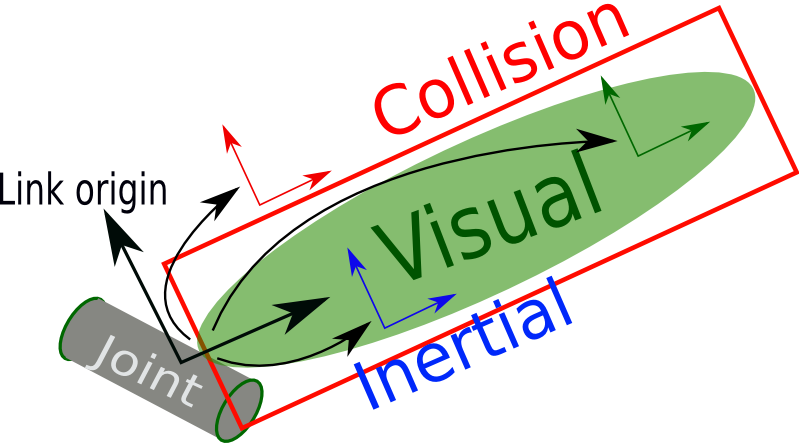
\includegraphics[width=0.60\textwidth]{chapter3/images/urdf_link.png}
	\caption{การอธิบาย link ใน URDF ไฟล์}
	\label{fig:urdf_link}
\end{figure}

\clearpage
\subsubsection*{Joint}
อีกส่วนที่สำคัญสำหรับการสร้างไฟล์หุ่นยนต์ด้วย URDF ก็คือ Joint tag โดย tag นี้จะอธิบายถึงความสัมพันธ์ระหว่างก้านต่อสองอัน
ส่วนนี้ไม่ได้มีเพียงแค่ทำข้อต่อให้เป็นแบบหมุนได้อย่างเดียว ยังมี Fix, Revolution, Linear และ Planar นอกเหนือจากนี้
เรายังสามารถที่จะเพิ่มองศาสูงสุดต่ำสุดของข้อต่อ รวมไปถึง dynamic properties ต่างๆ ตามที่เห็นดังรูปที่ \ref{fig:urdf_joint_code}
\begin{figure}[!ht]
\begin{Verbatim}[fontsize=\small]
<joint name="my_joint" type="floating">
	<origin xyz="0 0 1" rpy="0 0 3.1416"/>
	<parent link="link1"/>
	<child link="link2"/>
	<calibration rising="0.0"/>
	<dynamics damping="0.0" friction="0.0"/>
	<limit effort="30" velocity="1.0" lower="-2.2" upper="0.7"/>
	<safety_controller k_velocity="10" k_position="15" 
	soft_lower_limit="-2.0" soft_upper_limit="0.5"/>
</joint>
\end{Verbatim}
\caption{ตัวอย่าง joint ใน urdf}
	\label{fig:urdf_joint_code}
\end{figure}

เมื่อเรานำ Joint และ Link มารวมกันเราจะต้องพิจารณาว่ามีวางรูปแบบเป็นไปตามรูปที่ \ref{fig:urdf_joint}
โดยจะมีระยะระหว่างแกนของแต่ละข้อต่อกับก้านต่อ ชิ้นส่วนแรกของการสร้างไฟล์ URDF จะมีชื่อว่า base\_link
และเฟรม origin จะเป็นเฟรมอ้างอิง เมื่อเราต่อ Joint เข้ากับ Link จะเรียกก้านต่อที่เอามาติดว่า parent
โดยเฟรม origin ของข้อต่อจะอยู่จุดเดียวกับเฟรม origin ของก้านต่อ ในสถานะเดียวกันก้านต่อที่นำมาต่อจากข้อต่อ
เราจะเรียกว่า child และเฟรม origin ของก้านต่อ child จะอยู่ที่จุดเดียวกับเฟรม origin ของข้อต่อ

\begin{figure}[!ht]
	\centering
	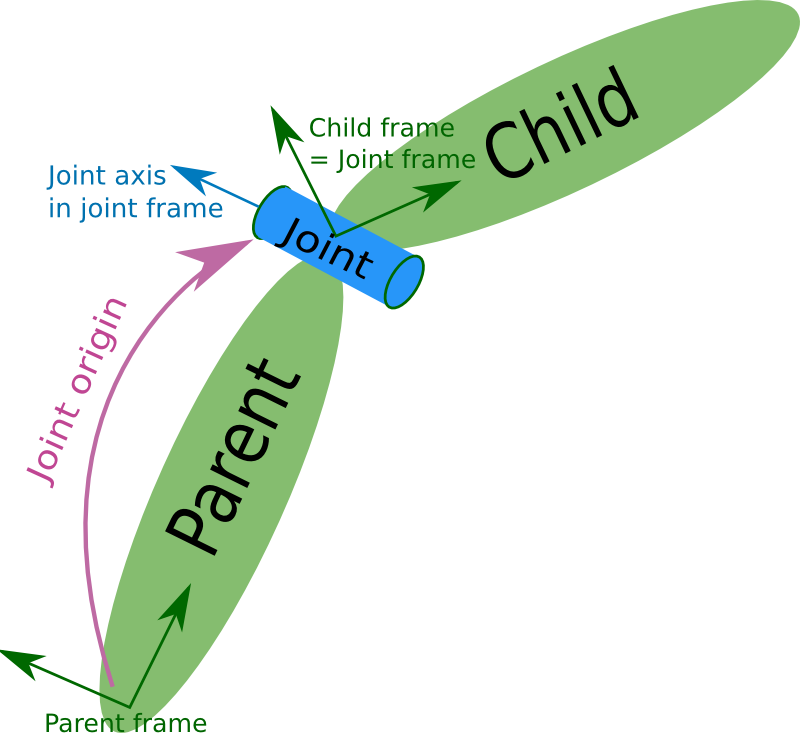
\includegraphics[width=0.55\textwidth]{chapter3/images/urdf_joint.png}
	\caption{การอธิบาย Joint ใน URDF ไฟล์}
	\label{fig:urdf_joint}
\end{figure}

%%%%%%%%%%%%%%%%%%%%%%%%%%%%%%%%%%%%%%%%%%%%%%%%%%%%%%%%%%%%%%%%%%%%%%%%%%%%%%%


%%%%%%%%%%%%%%%%%%%%%%%%%%%%%%%%%%%%%%%%%%%%%%%%%%%%%%%%%%%%%%%%%%%%%%%%%%%%%%%
%%%%%%%%%%%%%%%%%%%%%%%%%%%%%%%%%%%%%%%%%%%%%%%%%%%%%%%%%%%%%%%%%%%%%%%%%%%%%%%
\clearpage
\subsection{โครงสร้างการติดต่อสื่อสารระหว่าง Node ใน ROS}
การติดต่อสื่อสารกันภายใน ROS นั้นจะใช้การส่ง message หากัน ซึ่ง message แต่ละตัวก็จะใช้ในงานที่ต่างกัน
ตามระบบที่ต้องการส่ง จากรูปที่ \ref{fig:uthai_ros_node} เป็นโครงสร้างการส่งข้อมูลหากันของหุ่นยนต์ฮิวมานอยด์
ที่ผู้วิจัยได้ออกแบบไว้ โดยเริ่มจากผู้ใช้งานส่งตำแหน่งที่หุ่นยนต์จะต้องเดินไปไปยัง Node ที่ทำการคำนวณและสร้างตำแหน่งการวางเท้าของหุ่นยนต์
แล้วหลังจากนั้นจะส่งข้อมูลออกไปเป็น Path เส้นทางไปยัง Node ที่ทำการค้นหาตำแหน่งของ com, zmp ของหุ่นยนต์
เพื่อทำการควบคุมและสั่งการหุ่นยนต์ต่อไป

\begin{figure}[!ht]
	\centering
	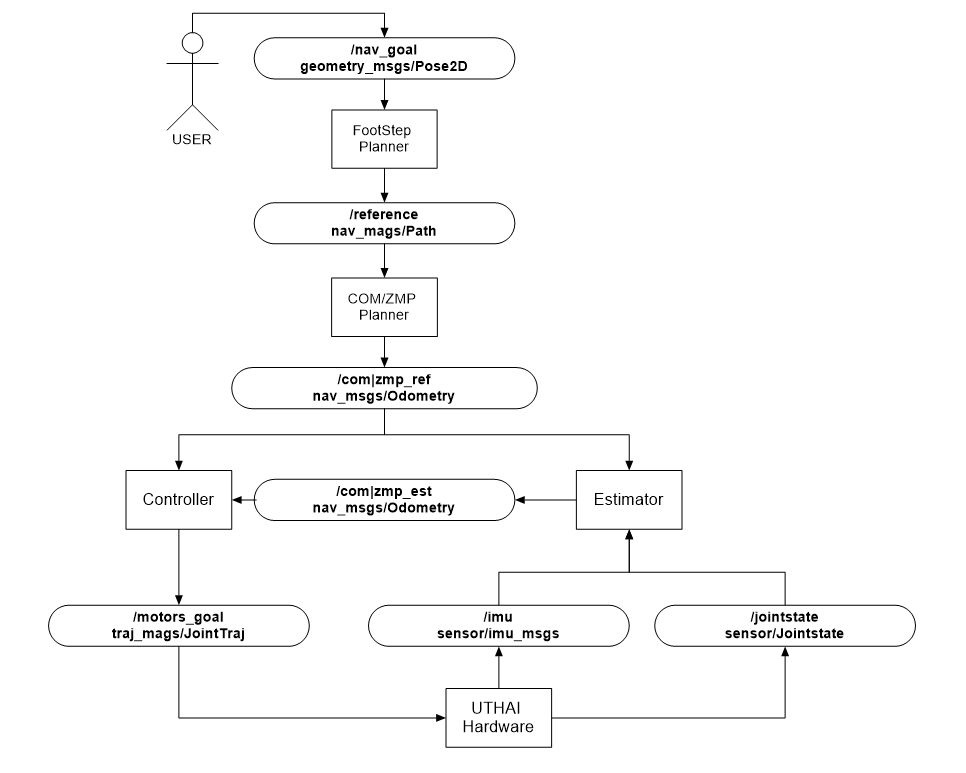
\includegraphics[width=\textwidth]{chapter3/images/uthai_ros_node.png}
	\caption{การติดต่อสื่อสารระหว่าง Node}
	\label{fig:uthai_ros_node}
\end{figure}

\subsubsection*{การบอกตำแหน่งและมุมเอียง}
การบอกตำแหน่งใน 3 มิติ Point คือการบอก $x$, $y$, $z$ และการบอกมุมเอียงจะใช้ Quaternion
ในการบอกโดยใช้ตัวแปรสี่ตัว คือ $x$,$y$,$z$,$w$ หากนำทั้งสองมารวมกันเราจะเรียกว่า Pose
\begin{table}[!ht]
	\centering
	\begin{tabular}{| c | c |}
		\hline
		\multicolumn{2}{|c|}{geometry\_msgs/Point}\\
		\hline
		float64 & x \\
		float64 & y \\
		float64 & z \\
		\hline
	\end{tabular}
	\caption{Message Geometry Point}
	\label{tab:geometry_point}
\end{table}
\begin{table}[!ht]
	\centering
	\begin{tabular}{| c | c |}
		\hline
		\multicolumn{2}{|c|}{geometry\_msgs/Quaternion}\\
		\hline
		float64 & x \\
		float64 & y \\
		float64 & z \\
		float64 & w \\
		\hline
	\end{tabular}
	\caption{Message Geometry Quaternion}
	\label{tab:geometry_quaternion}
\end{table}
\begin{table}[!ht]
	\centering
	\begin{tabular}{| c | c |}
		\hline
		\multicolumn{2}{|c|}{geometry\_msgs/Pose}\\
		\hline
		geometry\_msgs/Point & position \\
		geometry\_msgs/Quaternion & orientation \\
		\hline
	\end{tabular}
	\caption{Message Geometry Pose}
	\label{tab:geometry_pose}
\end{table}

\subsubsection*{การบอกความเร็วเชิงเส้นและเชิงมุม}
การบอกความเร็วเชิงเส้นใน 3 มิติ คือการบอกความเร็วตามแนวแกน $x$, $y$, $z$ และการบอกความเร็วเชิงมุม
คือการบอกความเร็วการหมุนรอบแกน $x$,$y$,$z$ หากนำทั้งสองมารวมกันเราจะเรียกว่า Twist
\begin{table}[!ht]
	\centering
	\begin{tabular}{| c | c |}
		\hline
		\multicolumn{2}{|c|}{geometry\_msgs/Vector3}\\
		\hline
		float64 & x \\
		float64 & y \\
		float64 & z \\
		\hline
	\end{tabular}
	\caption{Message Geometry Vector3}
	\label{tab:geometry_vector3}
\end{table}
\begin{table}[!ht]
	\centering
	\begin{tabular}{| c | c |}
		\hline
		\multicolumn{2}{|c|}{geometry\_msgs/Twist}\\
		\hline
		geometry\_msgs/Vector3 & linear \\
		geometry\_msgs/Vector3 & angular \\
		\hline
	\end{tabular}
	\caption{Message Geometry Twist}
	\label{tab:geometry_twist}
\end{table}

\subsubsection*{การบอกตำแหน่งและความเร็ว}
หากนำทั้งสองมารวมกันระกว่าง ตำแหน่ง (Pose) และความเร็ว (Twist) เราจะเรียกว่า Odometry
แต่ที่เพิ่มเข้ามาคือ Covariance ซึ่งอาจทำให้เกิดความสับสนได้
\begin{table}[!ht]
	\centering
	\begin{tabular}{| c | c |}
		\hline
		\multicolumn{2}{|c|}{nav\_msgs/Odometry}\\
		\hline
		std\_msgs/Header & header \\
		geometry\_msgs/PoseWithCovariance & pose \\
		geometry\_msgs/TwistWithCovariance & twist \\
		\hline
	\end{tabular}
	\caption{Message Navigation Odometry}
	\label{tab:nav_odometry}
\end{table}

\clearpage
\subsubsection*{ตำแหน่งของหุ่นยนต์}
การบอกตำแหน่งของหุ่นยนต์บนระนาบ 2 มิติ คือการบอก $x$, $y$ และ $\theta$
การบอกนั้นจะบอกว่าตำแหน่งที่หุ่นยนต์อยู่นั้นอยู่ตรงไหนหากเที่ยบกับแผนที่
รวมไปถึงตำแหน่งของหุ่นยนต์ที่ต้องการจะเดินไปด้วย ซึ่งอ้างอิงมาจากตำแหน่งเริ่มต้นของแผนที่ 
\begin{table}[!ht]
	\centering
	\begin{tabular}{| c | c |}
		\hline
		\multicolumn{2}{|c|}{geometry\_msgs/Pose2D}\\
		\hline
		float64 & x \\
		float64 & y \\
		float64 & theta \\
		\hline
	\end{tabular}
	\caption{Message Geometry Pose2D}
	\label{tab:geometry_pose2d}
\end{table}

\subsubsection*{ตำแหน่งการวางเท้าของหุ่นยนต์}
การจะให้หุ่นยนต์นำเท้าไปวางในตำแหน่งที่เราต้องการจากที่ได้จากการคำนวณนั้น
จะต้องบอกตำแหน่งและบอกมุมเอียงของจุดที่จะไป จากการสร้างจะได้เป็นรายการของเท้าซ้ายและขวา
โดยอิงจาก ตารางที่ \ref{tab:geometry_pose}
\begin{table}[!ht]
	\centering
	\begin{tabular}{| c | c |}
		\hline
		\multicolumn{2}{|c|}{nav\_msgs/Path}\\
		\hline
		std\_msgs/Header & header \\
		geometry\_msgs/PoseStamped[] & poses \\
		\hline
	\end{tabular}
	\caption{Message Navigation Path}
	\label{tab:nav_path}
\end{table}
\begin{table}[!ht]
	\centering
	\begin{tabular}{| c | c |}
		\hline
		\multicolumn{2}{|c|}{geometry\_msgs/PoseStamped}\\
		\hline
		std\_msgs/Header & header \\
		geometry\_msgs/Pose & pose \\
		\hline
	\end{tabular}
	\caption{Message Geometry PoseStamped}
	\label{tab:geometry_posestamped}
\end{table}

\subsubsection*{ตำแหน่งจุดศูนย์กลางมวลของหุ่นยนต์}
ใน Message นี้ใช้อยู่ 2 ที่คือ Message ที่ได้จากการวางแผนของ Node CoM Planner และ Node CoM Estimator
โดยทั้งสองจุดใช้ Message เหมือนกันส่งไปยัง Controller เพื่อควบคุมท่าทางต่างๆของหุ่นยนต์ต่อไป
Message ที่ใช้คือ Message จากตารางที่ \ref{tab:nav_odometry}
\begin{table}[!ht]
	\centering
	\begin{tabular}{| c | c |}
		\hline
		\multicolumn{2}{|c|}{nav\_msgs/Odometry}\\
		\hline
		std\_msgs/Header & header \\
		geometry\_msgs/PoseWithCovariance & pose \\
		geometry\_msgs/TwistWithCovariance & twist \\
		\hline
	\end{tabular}
	\caption*{Message Navigation Odometry}
\end{table}

\clearpage
\subsubsection*{การควบคุมข้อต่อของหุ่นยนต์}
ในการควบคุมข้อต่อแต่ละข้อของหุ่นยนต์ฮิวมานอยด์นั้นจะใช้ Message trjectory\_msgs/JointTrajectory
ซึ่งสามารถส่ง ตำแหน่ง ความเร็ว ความเร่ง และ แรงบิด ไปได้ ทำให้หากต้องการเปลี่ยนระบบใหม่สามารถทำได้โดยง่าย

\begin{table}[!ht]
	\centering
	\begin{tabular}{| c | c |}
		\hline
		\multicolumn{2}{|c|}{trajectory\_msgs/JointTrajectory}\\
		\hline
		std\_msgs/Header & header \\
		string[] & joint\_names \\
		trajectory\_msgs\_msgs/JointTrajectoryPoint[] & points \\
		\hline
	\end{tabular}
	\caption{Message Trajectory JointTrajectory}
	\label{tab:trajectory_jointrajectory}
\end{table}
\begin{table}[!ht]
	\centering
	\begin{tabular}{| c | c |}
		\hline
		\multicolumn{2}{|c|}{trajectory\_msgs/JointTrajectoryPoint}\\
		\hline
		float64[] & positions \\
		float64[] & velocities \\
  		float64[] & accelerations \\
  		float64[] & effort \\
  		duration & time\_from\_start \\
		\hline
	\end{tabular}
	\caption{Message Trajectory JointTrajectoryPoint}
	\label{tab:trajectory_jointrajectorypoint}
\end{table}

\subsubsection*{ค่าเซนเซอร์ข้อต่อของหุ่นยนต์}
ที่ข้อต่อของหุ่นยนต์ฮิวมานอยด์มีเซนเซอรที่เอาไว้ใช้ในการอ่านค่าตำแหน่ง ความเร็ว และแรง อยู่ด้วย
เราสามารถที่จะใช้ Message sensor\_msgs/JointState สำหรับอ่านค่าตำแหน่ง ความเร็ว แรง
ของตัวขับเคลื่อนแล้วส่งให้ Estimater Node ได้
\begin{table}[!ht]
	\centering
	\begin{tabular}{| c | c |}
		\hline
		\multicolumn{2}{|c|}{sensor\_msgs/JointState}\\
		\hline
		std\_msgs/Header & header \\
		float64[] & position \\
		float64[] & velocity \\
		float64[] & effort \\
		\hline
	\end{tabular}
	\caption{Message Sensor JointState}
	\label{tab:sensor_jointstate}
\end{table}

\subsubsection*{ค่าเซนเซอร์ฝ่าเท้าของหุ่นยนต์}
ที่ฝ่าเท้าของหุ่นยนต์ฮิวมานอยด์มีเซนเซอรที่เอาไว้ใช้ในการอ่าน แรงกดที่ฝ่าเท้า ใช้ในการเอามาบอกว่าเท้าสัมผัสพื้นหรือไม่
\begin{table}[!ht]
	\centering
	\begin{tabular}{| c | c |}
		\hline
		\multicolumn{2}{|c|}{geometry\_msgs/Wrench}\\
		\hline
		geometry\_msgs/Vector3 & force \\
		geometry\_msgs/Vector3 & torque \\
		\hline
	\end{tabular}
	\caption{Message Geometry Wrench}
	\label{tab:geometry_wrench}
\end{table}

\clearpage
\subsubsection*{ค่าเซนเซอร์ IMU ของหุ่นยนต์}
เซนเซอร์ IMU เป็นเซนเซอร์ที่เอาไว้ใช้ในการวัด ความเร็วเชิงมุม และ ความเร่งเชิงเส้น
หากนำทั้งคู่มารวมกันจะสามารถที่จะแปลงให้วัดมุมเอียงของเซนเซอร์ได้ โดยจะใช้ Message
std\_msgs/Imu ในการส่งให้ Node Estimator จากตัวหุ่นยนต์
\begin{table}[!ht]
	\centering
	\begin{tabular}{| c | c |}
		\hline
		\multicolumn{2}{|c|}{sensor\_msgs/Imu}\\
		\hline
		std\_msgs/Header & header \\
		geometry\_msgs/Quaternion & orientation \\
		float64[9] & orientation\_covariance \\
		geometry\_msgs/Vector3 & angular\_velocity \\
		float64[9] & angular\_velocity\_covariance \\
		geometry\_msgs/Vector3 & linear\_acceleration \\
		float64[9] & linear\_acceleration\_covariance \\
		\hline
	\end{tabular}
	\caption{Message Sensor Imu}
	\label{tab:sensor_imu}
\end{table}
\begin{table}[!ht]
	\centering
	\begin{tabular}{| c | c |}
		\hline
		\multicolumn{2}{|c|}{sensor\_msgs/MegneticField}\\
		\hline
		std\_msgs/Header & header \\
		geometry\_msgs/Vector3 & magnetic\_field \\
		float64[9] & magnetic\_field\_covariance \\
		\hline
	\end{tabular}
	\caption{Message Sensor MegneticField}
	\label{tab:sensor_megneticfield}
\end{table}
%%%%%%%%%%%%%%%%%%%%%%%%%%%%%%%%%%%%%%%%%%%%%%%%%%%%%%%%%%%%%%%%%%%%%%%%%%%%%%%
%%%%%%%%%%%%%%%%%%%%%%%%%%%%%%%%%%%%%%%%%%%%%%%%%%%%%%%%%%%%%%%%%%%%%%%%%%%%%%%